\documentclass[]{article}
\usepackage{lmodern}
\usepackage{amssymb,amsmath}
\usepackage{ifxetex,ifluatex}
\usepackage{fixltx2e} % provides \textsubscript
\ifnum 0\ifxetex 1\fi\ifluatex 1\fi=0 % if pdftex
  \usepackage[T1]{fontenc}
  \usepackage[utf8]{inputenc}
\else % if luatex or xelatex
  \ifxetex
    \usepackage{mathspec}
  \else
    \usepackage{fontspec}
  \fi
  \defaultfontfeatures{Ligatures=TeX,Scale=MatchLowercase}
\fi
% use upquote if available, for straight quotes in verbatim environments
\IfFileExists{upquote.sty}{\usepackage{upquote}}{}
% use microtype if available
\IfFileExists{microtype.sty}{%
\usepackage{microtype}
\UseMicrotypeSet[protrusion]{basicmath} % disable protrusion for tt fonts
}{}
\usepackage[margin=1in]{geometry}
\usepackage{hyperref}
\hypersetup{unicode=true,
            pdftitle={Final\_Project},
            pdfauthor={Aniket Naik Desai},
            pdfborder={0 0 0},
            breaklinks=true}
\urlstyle{same}  % don't use monospace font for urls
\usepackage{color}
\usepackage{fancyvrb}
\newcommand{\VerbBar}{|}
\newcommand{\VERB}{\Verb[commandchars=\\\{\}]}
\DefineVerbatimEnvironment{Highlighting}{Verbatim}{commandchars=\\\{\}}
% Add ',fontsize=\small' for more characters per line
\usepackage{framed}
\definecolor{shadecolor}{RGB}{248,248,248}
\newenvironment{Shaded}{\begin{snugshade}}{\end{snugshade}}
\newcommand{\AlertTok}[1]{\textcolor[rgb]{0.94,0.16,0.16}{#1}}
\newcommand{\AnnotationTok}[1]{\textcolor[rgb]{0.56,0.35,0.01}{\textbf{\textit{#1}}}}
\newcommand{\AttributeTok}[1]{\textcolor[rgb]{0.77,0.63,0.00}{#1}}
\newcommand{\BaseNTok}[1]{\textcolor[rgb]{0.00,0.00,0.81}{#1}}
\newcommand{\BuiltInTok}[1]{#1}
\newcommand{\CharTok}[1]{\textcolor[rgb]{0.31,0.60,0.02}{#1}}
\newcommand{\CommentTok}[1]{\textcolor[rgb]{0.56,0.35,0.01}{\textit{#1}}}
\newcommand{\CommentVarTok}[1]{\textcolor[rgb]{0.56,0.35,0.01}{\textbf{\textit{#1}}}}
\newcommand{\ConstantTok}[1]{\textcolor[rgb]{0.00,0.00,0.00}{#1}}
\newcommand{\ControlFlowTok}[1]{\textcolor[rgb]{0.13,0.29,0.53}{\textbf{#1}}}
\newcommand{\DataTypeTok}[1]{\textcolor[rgb]{0.13,0.29,0.53}{#1}}
\newcommand{\DecValTok}[1]{\textcolor[rgb]{0.00,0.00,0.81}{#1}}
\newcommand{\DocumentationTok}[1]{\textcolor[rgb]{0.56,0.35,0.01}{\textbf{\textit{#1}}}}
\newcommand{\ErrorTok}[1]{\textcolor[rgb]{0.64,0.00,0.00}{\textbf{#1}}}
\newcommand{\ExtensionTok}[1]{#1}
\newcommand{\FloatTok}[1]{\textcolor[rgb]{0.00,0.00,0.81}{#1}}
\newcommand{\FunctionTok}[1]{\textcolor[rgb]{0.00,0.00,0.00}{#1}}
\newcommand{\ImportTok}[1]{#1}
\newcommand{\InformationTok}[1]{\textcolor[rgb]{0.56,0.35,0.01}{\textbf{\textit{#1}}}}
\newcommand{\KeywordTok}[1]{\textcolor[rgb]{0.13,0.29,0.53}{\textbf{#1}}}
\newcommand{\NormalTok}[1]{#1}
\newcommand{\OperatorTok}[1]{\textcolor[rgb]{0.81,0.36,0.00}{\textbf{#1}}}
\newcommand{\OtherTok}[1]{\textcolor[rgb]{0.56,0.35,0.01}{#1}}
\newcommand{\PreprocessorTok}[1]{\textcolor[rgb]{0.56,0.35,0.01}{\textit{#1}}}
\newcommand{\RegionMarkerTok}[1]{#1}
\newcommand{\SpecialCharTok}[1]{\textcolor[rgb]{0.00,0.00,0.00}{#1}}
\newcommand{\SpecialStringTok}[1]{\textcolor[rgb]{0.31,0.60,0.02}{#1}}
\newcommand{\StringTok}[1]{\textcolor[rgb]{0.31,0.60,0.02}{#1}}
\newcommand{\VariableTok}[1]{\textcolor[rgb]{0.00,0.00,0.00}{#1}}
\newcommand{\VerbatimStringTok}[1]{\textcolor[rgb]{0.31,0.60,0.02}{#1}}
\newcommand{\WarningTok}[1]{\textcolor[rgb]{0.56,0.35,0.01}{\textbf{\textit{#1}}}}
\usepackage{graphicx,grffile}
\makeatletter
\def\maxwidth{\ifdim\Gin@nat@width>\linewidth\linewidth\else\Gin@nat@width\fi}
\def\maxheight{\ifdim\Gin@nat@height>\textheight\textheight\else\Gin@nat@height\fi}
\makeatother
% Scale images if necessary, so that they will not overflow the page
% margins by default, and it is still possible to overwrite the defaults
% using explicit options in \includegraphics[width, height, ...]{}
\setkeys{Gin}{width=\maxwidth,height=\maxheight,keepaspectratio}
\IfFileExists{parskip.sty}{%
\usepackage{parskip}
}{% else
\setlength{\parindent}{0pt}
\setlength{\parskip}{6pt plus 2pt minus 1pt}
}
\setlength{\emergencystretch}{3em}  % prevent overfull lines
\providecommand{\tightlist}{%
  \setlength{\itemsep}{0pt}\setlength{\parskip}{0pt}}
\setcounter{secnumdepth}{0}
% Redefines (sub)paragraphs to behave more like sections
\ifx\paragraph\undefined\else
\let\oldparagraph\paragraph
\renewcommand{\paragraph}[1]{\oldparagraph{#1}\mbox{}}
\fi
\ifx\subparagraph\undefined\else
\let\oldsubparagraph\subparagraph
\renewcommand{\subparagraph}[1]{\oldsubparagraph{#1}\mbox{}}
\fi

%%% Use protect on footnotes to avoid problems with footnotes in titles
\let\rmarkdownfootnote\footnote%
\def\footnote{\protect\rmarkdownfootnote}

%%% Change title format to be more compact
\usepackage{titling}

% Create subtitle command for use in maketitle
\providecommand{\subtitle}[1]{
  \posttitle{
    \begin{center}\large#1\end{center}
    }
}

\setlength{\droptitle}{-2em}

  \title{Final\_Project}
    \pretitle{\vspace{\droptitle}\centering\huge}
  \posttitle{\par}
    \author{Aniket Naik Desai}
    \preauthor{\centering\large\emph}
  \postauthor{\par}
      \predate{\centering\large\emph}
  \postdate{\par}
    \date{2019-06-16}


\begin{document}
\maketitle

\hypertarget{questions-for-exploratory-data-analysis-of-gapminder-dataset}{%
\subsection{Questions for Exploratory Data Analysis of gapminder
dataset}\label{questions-for-exploratory-data-analysis-of-gapminder-dataset}}

\begin{enumerate}
\def\labelenumi{\arabic{enumi}.}
\tightlist
\item
  At the same income level, does increase in average life expectancy
  vary based on region?
\item
  Has average life expectancy increased in all regions at the same rate
  over the years?
\item
  At what income level does the increase in life expectancy stop
  increasing for the various regions?
\end{enumerate}

\hypertarget{data-description}{%
\section{Data Description}\label{data-description}}

We have 41284 observations and 6 variables. Two variables of the six
variables are categorical and four variables are continous.

\hypertarget{type-of-data-variables}{%
\subsection{Type of Data Variables}\label{type-of-data-variables}}

Country and region are categorical variables with 197 levels (countries)
and 6 levels (regions) respectively. Year, Population, Life, and income
are numeric variables. Life variable is the life expectancy of the
population while income is calculated as gdp per capita.

\hypertarget{missing-values}{%
\subsection{Missing Values}\label{missing-values}}

We have missing values in population and income variables. The missing
population values were filled with the population count at the start of
the decade. We have 2341 NA values in the income variable spread over 14
countries. These countries do not have any income values recorded in the
dataset hence we are not able to compute any values to replace the NA
values. Hence, in any calculation involving income we will ignore the
following countries French Guiana, Guadeloupe, Martinique, Netherlands
Antilles, Virgin Islands (U.S.), French Polynesia, Guam, New Caledonia,
Tokelau, Ã\ldots{}land, Channel Islands, Western Sahara, Mayotte,
Reunion.

\hypertarget{data-dispersion}{%
\subsection{Data Dispersion}\label{data-dispersion}}

We have data about 197 countries which are divided into 6 regions. Our
data has been gathered over 215 years starting from 1800 up till 2015 .
The population of all countries changed over time with China from China
region having the highest population in 2015 and Marshall Islands from
East Asia \& Pacific region having the lowest population in 2015.

The 6 regions do not have equal number of countries with 3 having the
highest number of countries (51) and 5 having the lowest number of
countries (8).

Life expectacy has varied greatly with Fiji, French Polynesia, and Samoa
showing a low of 1 year life expectacy in the years 1875, 1918, and 1918
respectively. With Andorra showing the highest life expectacy of 84.1 in
2015. The overall mean for life was 71.7634831 in 2015. Regionwise this
was

Income has range has been very wide with United Arab Emirates having the
peak income of 182668 in the year 1980. In the year 2015, Kuwait had the
highest income of 132877 while Somalia had the lowest income of 624 in
2015.

\hypertarget{outliers}{%
\subsection{Outliers}\label{outliers}}

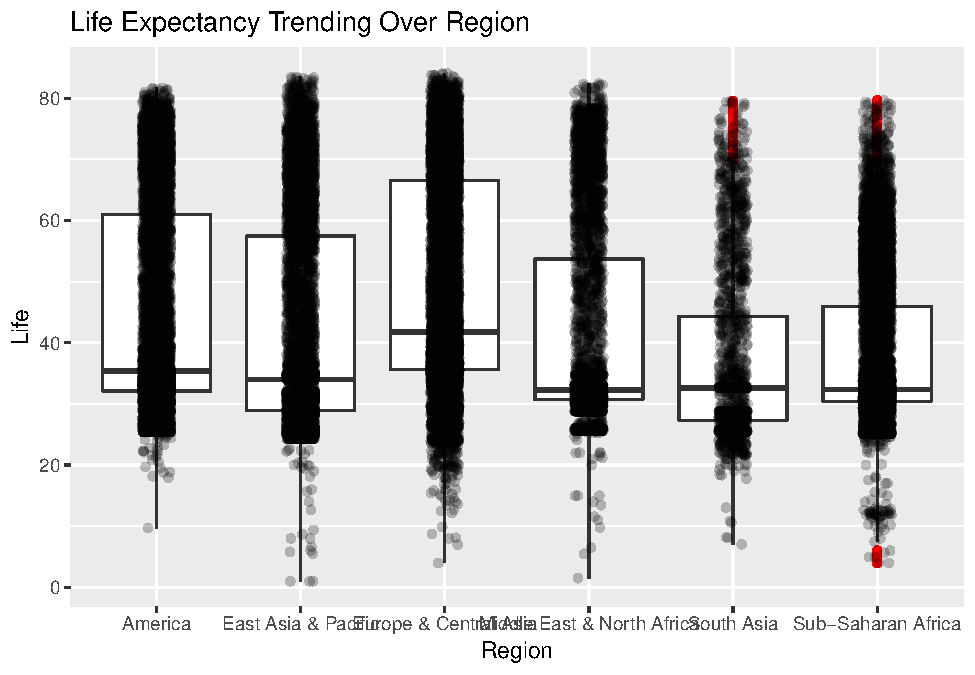
\includegraphics{Final_Project_files/figure-latex/Outliers-1.pdf}
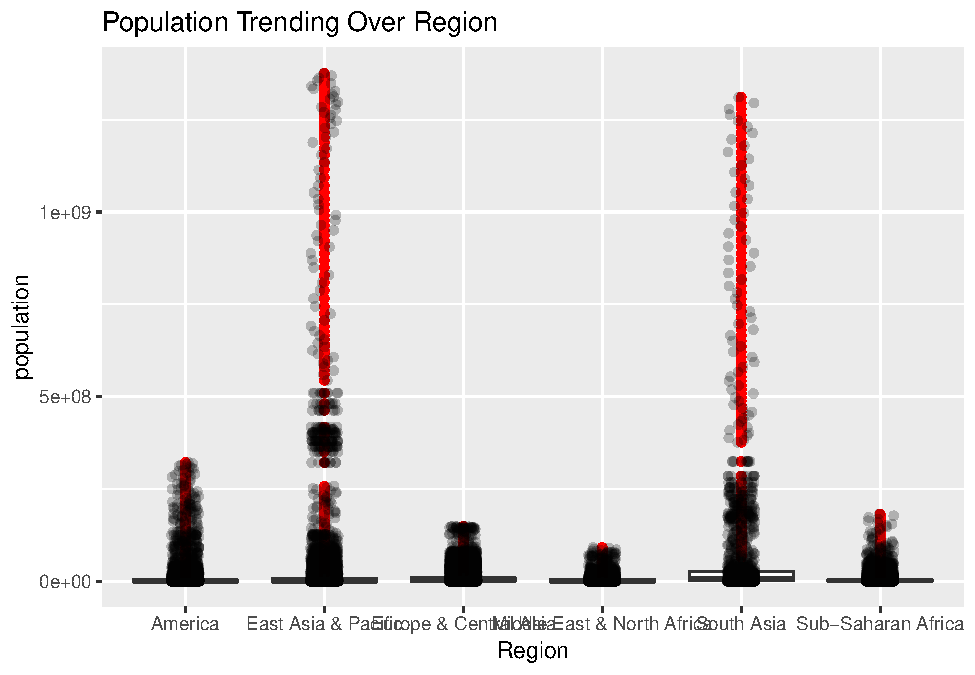
\includegraphics{Final_Project_files/figure-latex/Outliers-2.pdf}
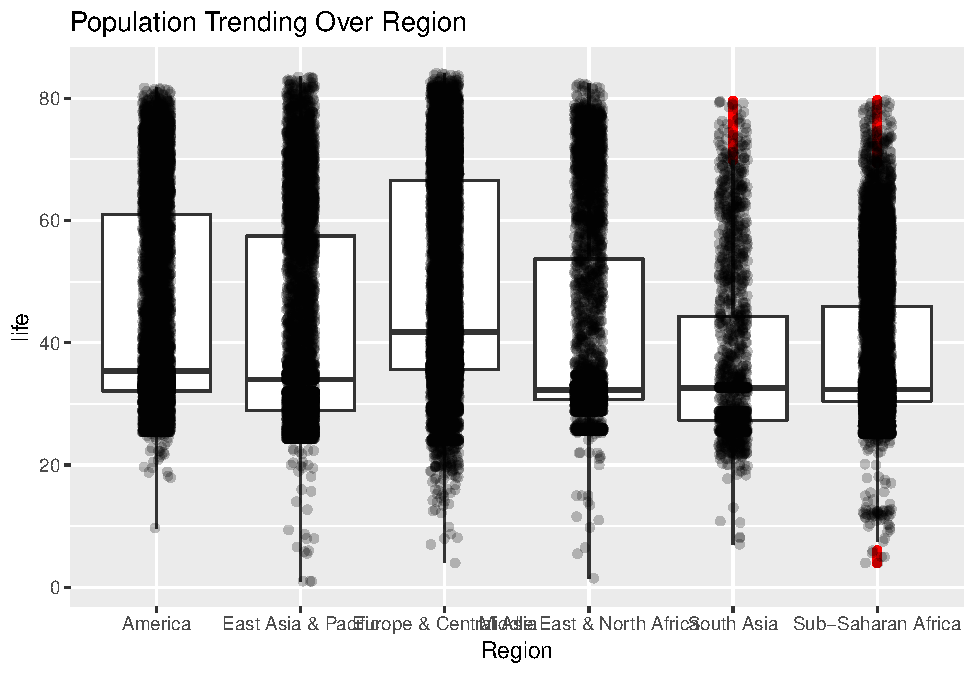
\includegraphics{Final_Project_files/figure-latex/Outliers-3.pdf} We see
that we have a few outliers in population and income but we can ignore
these are we will do a log scaling to take care of it. Life does not
have any large outliers that we need to do any trasformation.

\hypertarget{data-preprocessing}{%
\subsection{Data Preprocessing}\label{data-preprocessing}}

We saw in our initial analysis that we have a very wide range for
population and income. This is detrimental to our analysis as values
from a few countries will cause a heavy bias and potentially give us
wrong observations/results. Hence, we will log transform the population
and income variables. This will help us lower the range and weight of
the outliers.

\hypertarget{data-wrangling}{%
\subsection{Data Wrangling}\label{data-wrangling}}

\hypertarget{exploratory-data}{%
\subsection{Exploratory Data}\label{exploratory-data}}

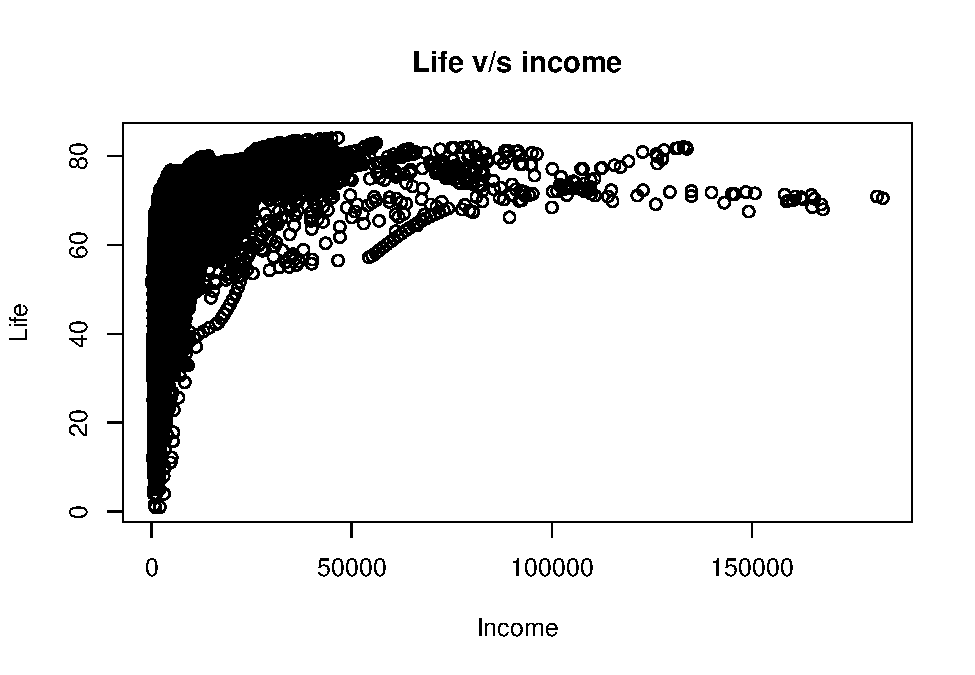
\includegraphics{Final_Project_files/figure-latex/Plots-1.pdf}
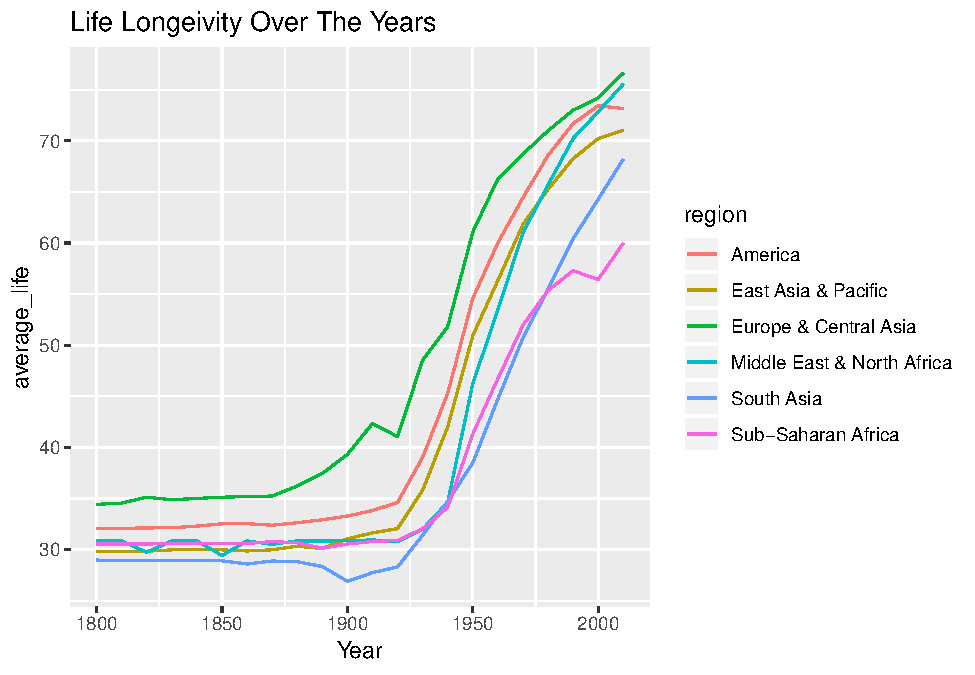
\includegraphics{Final_Project_files/figure-latex/Plots-2.pdf} We see a
definite correlation between life and income levels, we start seeing
some oddities when we go part \$50,000 where the increase in income has
less effect on the increase in life expectancy.

\hypertarget{clustering}{%
\subsubsection{Clustering}\label{clustering}}

We have done the custering for data in the year 2015. When doing
clustering we will need to omit the rows with missing values in income
field.

\hypertarget{kmeans}{%
\section{Kmeans}\label{kmeans}}

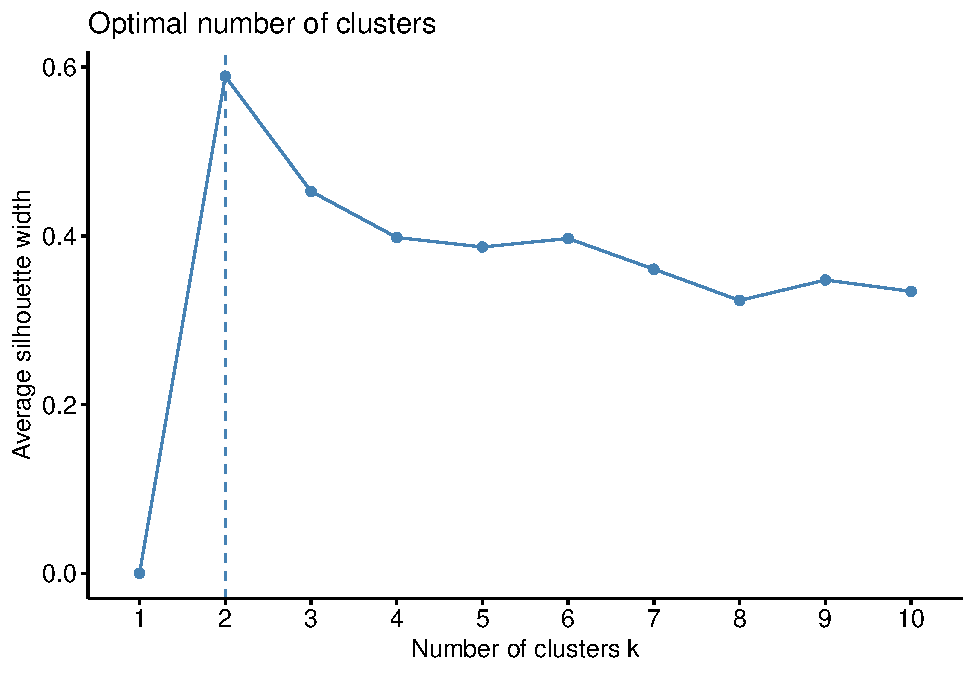
\includegraphics{Final_Project_files/figure-latex/Clustering Kmeans-1.pdf}
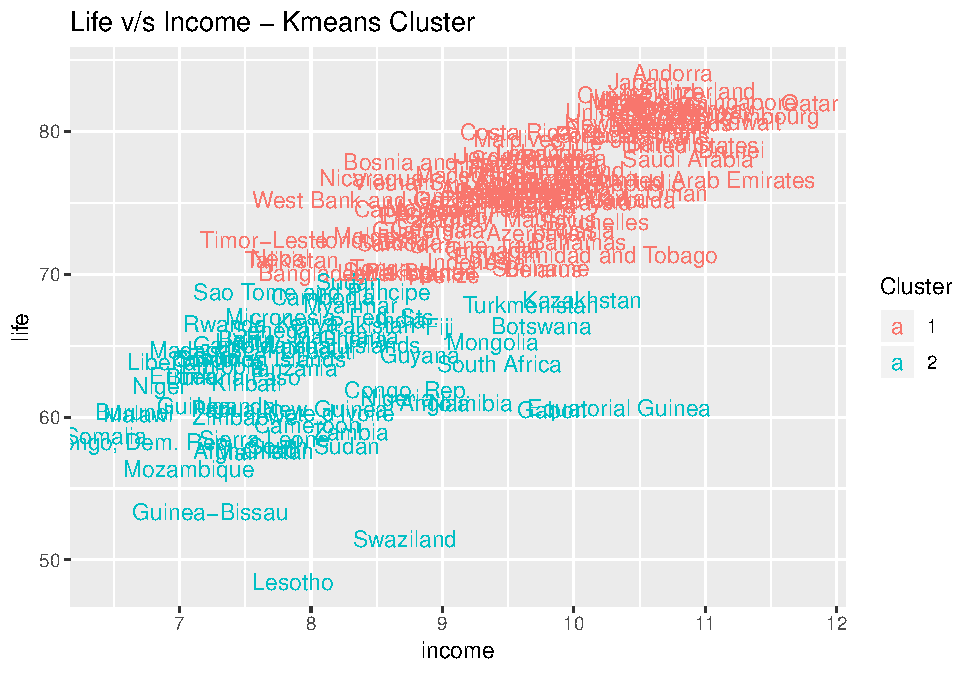
\includegraphics{Final_Project_files/figure-latex/Clustering Kmeans-2.pdf}
We choose 2 clusters based on silhouette method. We see that in Kmeans
Cluster the countries are more or less divided based on the life
expectacy in 2015. The cutoff seems to be near 70 years of life
expectancy. This also points to an interesting fact that richer
countries don't actually live longer than poorer countries.

\hypertarget{hierarchical-cluster}{%
\section{Hierarchical Cluster}\label{hierarchical-cluster}}

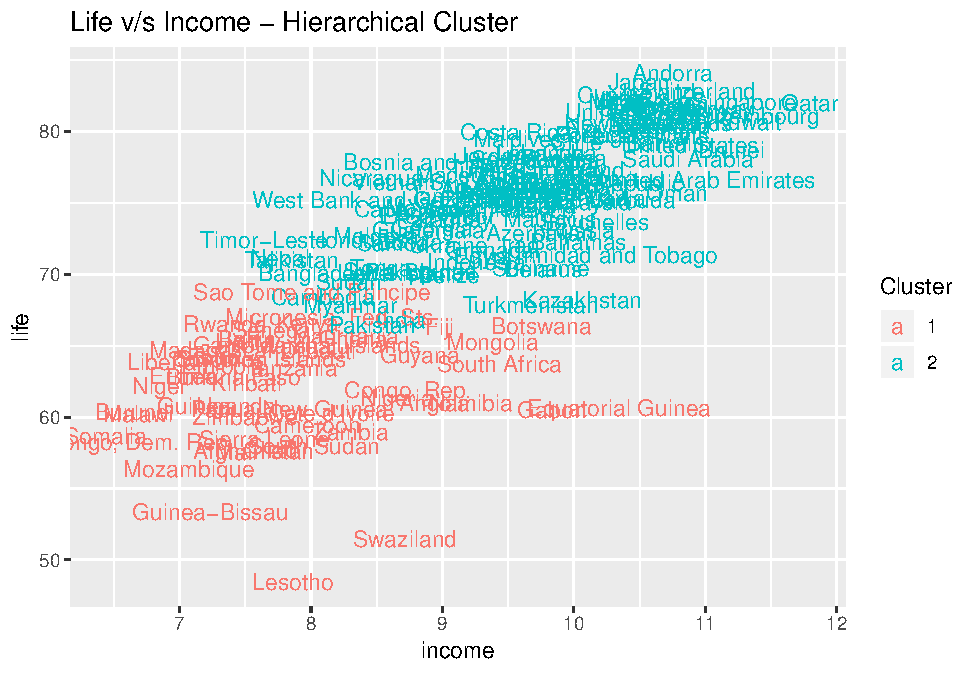
\includegraphics{Final_Project_files/figure-latex/Clustering Hierarchical-1.pdf}
We choose 2 clusters based on silhouette method. We see similar results
with the cluster being separated long life variable but here the cutoff
seems to be slightly lower than 70 years.

\hypertarget{summary}{%
\subsection{Summary}\label{summary}}

We see that at the same income level, increase in average life
expectancy varies based on region. It increases sharply in 1950's for
all regions but in different levels. Average life expectancy has not
increased in all regions at the same rate over the years. Middle east
region has lead the increase since 1950. At 50,000 income level the
increase in life expectancy stop increasing as sharply and we see that
the growth is minimal.

\begin{Shaded}
\begin{Highlighting}[]
\KeywordTok{warnings}\NormalTok{()}
\end{Highlighting}
\end{Shaded}

\begin{verbatim}
## NULL
\end{verbatim}


\end{document}
